% 前置知识
看左图里兔子的下巴和尾巴。点光源照不到的一侧几乎融进黑色背景。地面也受到了照明，其中一部分光从地面反射回来，能照到兔子的背光面。把单独算出的这部分光（中图）加到左图上，右图里就能辨出尾巴的轮廓。

\begin{center}
\begin{tabularx}{\linewidth}{@{}XXX@{}}
\centering\arraybackslash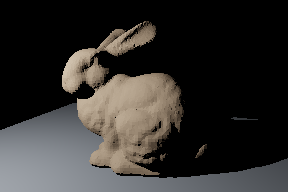
\includegraphics[width=\linewidth]{figures/bunny-direct.png} &
\centering\arraybackslash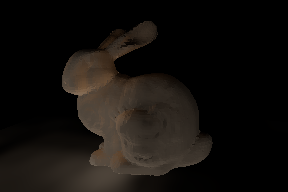
\includegraphics[width=\linewidth]{figures/bunny-bounce.png} &
\centering\arraybackslash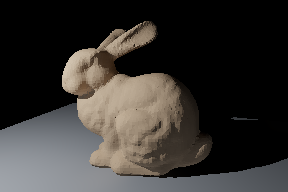
\includegraphics[width=\linewidth]{figures/bunny-combined.png}\\[-1pt]
\centering\arraybackslash\small 直接光 &
\centering\arraybackslash\small DDGI 间接光 &
\centering\arraybackslash\small 两者相加
\end{tabularx}\\[2pt]
{\footnotesize\color{quiet}Stanford Bunny，Redflag Vulkan，$288\times192$。探针计算一次漫反射，连续更新 8 帧；三张图使用同一曝光。}
\end{center}

要估算各处能收到多少反射光，可以在场景中布置一组探针，让它们从各自的位置向四周取样。给兔子着色时，就从附近的探针读取间接光。移到 Sponza 的走廊，还要当心墙另一侧的探针。探针会记下光线走多远碰到了表面，查询时这份记录能帮助判断两者之间是否隔着墙。

% 公式推导
GAMES101 的余弦项可以用一束平行光照在斜纸上的覆盖面积来理解。把单位方向 $\omega$ 与单位法线 $n$ 做点积，得到 $\cos\theta$。对墙面上半球的来光按这个值加权，就是辐照度 $E$。在 PBRT 的漫反射模型中，反射率为 $\rho$ 的墙把这些光转换为出射辐亮度 $L_o=\rho E/\pi$。现在把取样方向的密度选成 $\cos\theta/\pi$，代入采样估计式，余弦和 $\pi$ 正好抵消。此处 $\rho$ 对应 $(1-m)c$，一块纯金属板的 $m=1$，不把它的底色加进漫反射。探针累加追踪得到的来光，平均值直接估计 $E/\pi$。

% 公式
\[
 E(n)=\int_{\Omega^+}L_i(\omega)(n\cdot\omega)\,d\omega,\qquad
 \widehat{E/\pi}=\frac1N\sum_j L_i(\omega_j).
\]
探针还保存距离均值 $\mu$ 和距离平方的均值 $\mu_2$。方差 $v=\max(\mu_2-\mu^2,\epsilon)$。查询点距离探针 $d$，当 $d$ 比已见表面更远时，用 $v/[v+\max(d-\mu,0)^2]$ 降低权重。这是由距离统计得到的可见性近似。墙的厚度和遮挡方向如果没被六个方向充分分辨，仍然会漏光。
把一支探针放在薄墙旁，向左射出的光很快撞墙，向右却能穿过整间屋子。NVIDIA 的 RTXGI 给每支探针存随方向变化的光量和距离。Redflag 把方向合并到六个主轴，再按方向插值。较小的记录给得出大致的反光，斜对着墙时，墙前与墙后的距离也可能被平均在一起。\href{https://github.com/NVIDIAGameWorks/RTXGI-DDGI/blob/main/docs/Algorithms.md}{NVIDIA 的 DDGI 算法说明}
\pair{profiling/gi/ddgi.png}{六方向探针插值}{profiling/gi/indirect-reference.png}{两组独立 512 spp 的平均}
\clearpage
% 逐行伪代码
\subsection{用探针照亮柱面}
\noindent{\small\color{quiet}按 GLSL 整理的伪代码\quad\href{run:../../Redflag/src/Redflag/Renderer/GI/Shaders/GI.comp}{\texttt{GI.comp}}}\par\nopagebreak
\begin{lstlisting}[escapeinside={(*@}{@*)}]
for probe, face in grid * sixDirections:
    for ray in cosineWeightedHemisphere(face):
        hit, distance = traceFrom(probe, ray)
        radiance += directLightingAt(hit)
        moments += (distance, distance * distance)
    storeOrBlend(probe, face, radiance / N, moments / N)
for pixel in visibleSurfaces:
    for probe in eightCornersAround(pixel.position):
        weight = trilinearWeight * visibilityWeight * facingWeight
        sum += weight * readIrradianceOverPi(probe, pixel.normal)
        total += weight
    (*@{\footnotesize\color{quiet}先将附近探针的光归一化，再乘本像素的反射率。}@*)
    output = pixel.albedo * sum / max(total, epsilon)
\end{lstlisting}
第一次更新用这一帧的结果，之后以 0.2 的比例接纳新值。三线性插值的几何权重只表示离哪个角近；查询点朝向以及隔墙的概率另算，最后按实际权重和归一化。

0.2 来自响应速度的取舍。某次观测经过三次更新，留下的比例为 $0.8^3=0.512$，约一半；提高这个系数，开灯后的变化更快，单帧噪声也更容易显出来。$12\times6\times7$ 是这个长走廊使用的网格数量。与其直接照搬到新场景，可以先用各轴长度除以对应数量，看看两探针之间是否塞进了一整堵薄墙。

% 接口与数据结构
\begin{fields}
\texttt{Probe.light} & 每探针六个主轴方向各存一份 RGB 的 $E/\pi$，查询法线按与各轴夹角的余弦平方混合。\\
\texttt{Probe.moments} & 存距离与距离平方的平均。相同的网格索引能找到光量和遮挡信息。\\
\texttt{Render(DDGI, 16)} & 先更新探针，再给当前可见表面插值。基准中每个方向用 16 条射线。\\
\end{fields}

% 验证标准
$12\times6\times7$ 个探针经过 8 帧更新，可见像素的线性 RGB 均方误差为 \measured{ddgi-mse}。图像的通道均值是 \measured{ddgi-mean_rgb}，参考为 \measured{reference-mean}。亮度均值之间的差距在空间插值后仍存在。比较同一墙角的距离矩、探针位置和参考图，可以继续定位误差。这组对照只计算一次漫反射。接下来让墙面接收上一轮探针记下的光，再观察光传到第二面墙时发生的变化。
